%
\documentclass[11pt]{article}

% The usual packages
\usepackage{booktabs}
\usepackage{array}
\usepackage{subcaption}

\usepackage{fullpage}
\usepackage{breakcites}
\usepackage{setspace}
\usepackage{endnotes}
%\usepackage{float} % can't use with floatrow
\usepackage{amsmath}
\usepackage{amsfonts}
\usepackage{amssymb}
\usepackage{rotating}
\usepackage{longtable}
\usepackage{microtype}
\usepackage{graphicx}
\usepackage{hyperref}
%\usepackage[usenames,dvipsnames]{color}
\usepackage{url}
\usepackage{natbib}
\usepackage{framed}
\usepackage{epigraph}
\usepackage{lipsum}
\usepackage{textcomp} % for \textrightarrow
%\usepackage{dcolumn}
%\restylefloat{table}
\bibpunct{(}{)}{;}{a}{}{,}

% Set paragraph spacing the way I like
\parskip=0pt
\parindent=20pt

%\usepackage{helvet}
\usepackage[labelfont={bf}, margin=0cm, font=small, skip=0pt]{caption}

\newcommand\numberthis{\addtocounter{equation}{1}\tag{\theequation}}

% Define mathematical results
\newtheorem{lemma}{Lemma}
\newtheorem{proposition}{Proposition}
\newtheorem{theorem}{Theorem}
\newtheorem{claim}{Claim}
\newenvironment{proof}[1][Proof]{\begin{trivlist}
\item[\hskip \labelsep {\bfseries #1}]}{\end{trivlist}}
\newenvironment{definition}[1][Definition]{\begin{trivlist}
\item[\hskip \labelsep {\bfseries #1}]}{\end{trivlist}}
\newenvironment{example}[1][Example]{\begin{trivlist}
\item[\hskip \labelsep {\bfseries #1}]}{\end{trivlist}}
\newenvironment{remark}[1][Remark]{\begin{trivlist}
\item[\hskip \labelsep {\bfseries #1}]}{\end{trivlist}}
\DeclareMathOperator*{\argmin}{arg\,min}
\DeclareMathOperator{\med}{med}
\DeclareMathOperator*{\E}{\text{E}}
%\DeclareMathOperator*{\Pr}{\text{Pr}}

%Set up fonts the way I like
%\usepackage{tgpagella}
%\usepackage[T1]{fontenc}
%\usepackage[bitstream-charter]{mathdesign}

%% Baskervald
\usepackage[lf]{Baskervaldx} % lining figures
\usepackage[bigdelims,vvarbb]{newtxmath} % math italic letters from Nimbus Roman
\usepackage[cal=boondoxo]{mathalfa} % mathcal from STIX, unslanted a bit
\renewcommand*\oldstylenums[1]{\textosf{#1}}

%\usepackage[T1]{fontenc}
%\usepackage{newtxtext,newtxmath}

% A special command to create line break in table cells
\newcommand{\specialcell}[2][c]{%
 \begin{tabular}[#1]{@{}c@{}}#2\end{tabular}}

%% Set up lists the way I like
% Redefine the first level
\renewcommand{\theenumi}{\arabic{enumi}.}
\renewcommand{\labelenumi}{\theenumi}
% Redefine the second level
\renewcommand{\theenumii}{\alph{enumii}.}
\renewcommand{\labelenumii}{\theenumii}
% Redefine the third level
\renewcommand{\theenumiii}{\roman{enumiii}.}
\renewcommand{\labelenumiii}{\theenumiii}
% Redefine the fourth level
\renewcommand{\theenumiv}{\Alph{enumiv}.}
\renewcommand{\labelenumiv}{\theenumiv}
% Eliminate spacing around lists
\usepackage{enumitem}
\setlist{nolistsep}

% Create footnote command so that my name
% has an asterisk rather than a one.
\long\def\symbolfootnote[#1]#2{\begingroup%
\def\thefootnote{\fnsymbol{footnote}}\footnote[#1]{#2}\endgroup}
%\usepackage{footmisc}
%\renewcommand{\thefootnote}{\symbolfootnote{footnote}}

% Create the colors I want
\usepackage{color, xcolor}
\definecolor{color1}{RGB}{217,95,2}  % orange
\definecolor{color2}{RGB}{27,158,119}  % green
\definecolor{color3}{RGB}{117,112,179}  % purple

% for colored \left( and \right)
\newcommand{\cleft}[2][.]{%
  \begingroup\colorlet{savedleftcolor}{.}%
  \color{#1}\left#2\color{savedleftcolor}%
}
\newcommand{\cright}[2][.]{%
  \color{#1}\right#2\endgroup
}

% for drawing arrows
\usepackage{tikz}
\usetikzlibrary{calc,shapes}

\newcommand{\tikzmark}[1]{\tikz[overlay,remember picture] \node (#1) {};}
\newcommand{\DrawBox}[2]{%
  \begin{tikzpicture}[overlay,remember picture]
    \draw[->,shorten >= 6pt, shorten <= 2pt, out=-90, in=90, distance=1.2cm, color2, thick] (MarkA.east) to (MarkB.east);
    \draw[->,shorten >= 6pt, shorten <= 2pt, out=-90, in=90, distance=1cm, color2, thick] (MarkC.west) to (MarkD.east);
  \end{tikzpicture}
}

% remarks by equations
\newcommand{\justif}[2]{&{#1}&\text{#2}}


% set up pdf
\hypersetup{
pdftitle={}, % title
pdfauthor={Carlisle Rainey}, % author
pdfkeywords={bias} {first difference} {marginal effect} {quantities of interest} {maximum likelihood}
pdfnewwindow=true, % links in new window
colorlinks=true, % false: boxed links; true: colored links
linkcolor=black, % color of internal links
citecolor=black, % color of links to bibliography
filecolor=blue, % color of file links
urlcolor=blue % color of external links
}

% section headers
%\usepackage[scaled]{helvet}
%\renewcommand\familydefault{\sfdefault}
%\usepackage[T1]{fontenc}
%\usepackage{titlesec}
%\titleformat{\section}
%  {\normalfont\sffamily\Large\bfseries}
%  {\thesection}{1em}{}
%\titleformat{\subsection}
%  {\normalfont\sffamily\large\bfseries}
%  {\thesection}{1em}{}
%  \titleformat{\subsubsection}
%  {\normalfont\sffamily\bfseries}
%  {\thesection}{1em}{}

% enable comments in pdf
\newcommand{\dtk}[1]{\textcolor{blue}{#1}}
\newcommand{\ctk}[1]{\textcolor{red}{#1}}

\begin{document}

\begin{center}

{\LARGE \textbf{Unnecessary Bias}}\\\vspace{2mm}
{ \textbf{Do Not Use the Average of Simulations to Estimate Quantities of Interest}}\symbolfootnote[1]{All computer code necessary for replication is available on \href{https://github.com/carlislerainey/unnecessary}{GitHub}.}

\vspace{5mm}

Carlisle Rainey\symbolfootnote[2]{Carlisle Rainey is Assistant Professor of Political Science, Texas A\&M University, 2010 Allen Building, College Station, TX, 77843. (\href{mailto:crainey@tamu.edu}{crainey@tamu.edu}).}

\vspace{5mm}

Holger L. Kern\symbolfootnote[3]{Holger L. Kern is Assistant Professor of Political Science, Florida State University, 541 Bellamy, Tallahassee, FL, 32306. (\href{mailto:hkern@fsu.edu}{hkern@fsu.edu}).}

\vspace{1cm}

\today
\end{center}

\vspace{5mm}

% Abstract
{\centerline{\textbf{Abstract}}}
\begin{quote}\noindent
Following \cite{KingTomzWittenberg2000}, researchers commonly convert coefficient estimates into an estimate of the quantity of interest using the average of simulations.
However, other researchers simply use the invariance property of maximum likelihood estimates to directly convert the model coefficient estimates into the quantity of interest.
These approaches are not equivalent, yet researchers rarely justify their choice.
I show that the average of simulations can introduce substantial bias compared to the maximum likelihood estimate.
In general, when reporting point estimates of the quantity of interest, researchers should report the maximum likelihood estimate, not the average of the simulations.
 \end{quote}

% Add quote to first page
% \epigraph{}

%\begin{center}
%Manuscript word count:
%\end{center}

% Remove page number from first page
\thispagestyle{empty}

% Start main text
%\newpage
%\doublespace
\onehalfspace
%\section*{Introduction}

Political scientists now routinely employ maximum likelihood (ML) estimators to model a wide variety of dependent variables. Examples include probit, logit, and rare events logistic regression (King and Zeng 2001) for binary outcomes; ordered logit and probit for ordered categorical outcomes; multinomial logit and probit for unordered categorical outcomes; Poisson and negative binomial regression for count data, and beta regression for fractions (Paolino 2001). Numerous additional ML estimators could be listed here, many of them proposed by political scientists and regularly used in political science research. What all of these estimators have in common is that model coefficients are not directly informative about the substantive impact of changes in predictors on the dependent variable.

\cite{KingTomzWittenberg2000} noticeably improved quantitative research in political science by urging political scientists to focus on substantively meaningful {\it quantities of interest} such as predicted probabilities, expected counts, marginal effects, and first differences. Before the publication of \cite{KingTomzWittenberg2000}, it was common for political scientists to present lengthy tables of estimated model coefficients from non-linear models, with little or no attention paid to the substantive interpretation of the results beyond the sign and statistical significance of the model coefficients. Moreover, when researchers did report quantities of interest they often failed to provide valid measures of uncertainty for them. Expectations about how empirical results should be presented changed after the publication of \cite{KingTomzWittenberg2000} and the availability of easy-to-use software for Stata (CLARIFY) and \texttt{R} (Zelig). According to the Web of Science, by January 2018 \cite{KingTomzWittenberg2000} has been cited 1,097 times, making it the fourth most-cited methodology article in political science, at least among those published in the \textit{American Political Science Review}, the \textit{American Journal of Political Science}, and \textit{Political Analysis}. Moreover, it is the second most-cited article \textit{overall} in the \textit{American Journal of Political Science}, falling just $56$ citations short of \cite{BeckKatzTucker1998}. Google Scholar suggests that \cite{KingTomzWittenberg2000} has as many as 3,598 citations, that \cite{TomzWittenbergKing2003}, which provides an overview of the CLARIFY software, has as many as 1,437, and that Imai, King, and Lau (2008), which proposes a common framework for statistical analysis and software development centered on Zelig, has as many as 318. In short, the valuable advice offered by \cite{KingTomzWittenberg2000} has been incredibly influential, not only in political science but across the social sciences.

In addition to highlighting the importance of reporting substantively meaningful quantities of interest, a major contribution of \cite{KingTomzWittenberg2000} was to popularize {\it stochastic simulation} to compute quantities of interest and associated measures of statistical uncertainty. Stochastic simulation repeatedly draws model coefficients from their asymptotic multivariate normal sampling distribution, transforms them into quantities of interest (such as marginal effects or predicted probabilities), and then summarizes the distribution of simulated estimates by reporting its mean and standard error.

Our paper addresses one particular aspect of \cite{KingTomzWittenberg2000}'s advice: to use the mean of the simulated quantities of interest as the point estimator for the quantity of interest. As we will show both analytically and empirically, this choice is suboptimal in that it can introduce unnecessary finite sample bias into estimates of quantities of interest. Instead, we propose that political scientists compute quantities of interest based on the ML {\it invariance} property, which, as we will show, generally results in less finite sample bias. Informally speaking, the ML invariance property says that we can estimate the function of a parameter by estimating the parameter using ML and then applying the function to the estimate (\citealt[pp. 75-76]{King1989}, and \citealt[pp. 320-321]{CasellaBerger2002}).

More formally, suppose a researcher uses ML to estimate a statistical model in which $y_i \stackrel{iid}{\sim} f(\theta_i)$, where $i \in \{1,\ldots, N\}$ and $f$ represents a probability distribution. The parameter $\theta_i$ is connected to a design matrix $X$ of $k$ explanatory variables and a column of ones by a link function $g$, so that $g(\theta_i) = X_i\beta$, where $\beta \in \mathbb{R}^{k+1}$ represents a vector of coefficients with length $k + 1$. The researcher uses maximum likelihood to compute estimates $\hat{\beta}^{\text{mle}}$ for the parameter vector $\beta$.\footnote{Note that we adopt a frequentist perspective, so $\hat{\beta}^{\text{mle}}$ represents a \emph{random variable} that varies across samples.} We refer to the function that transforms model coefficients into quantities of interest as $\tau(\cdot)$. For a probit model, for example, $\tau(\cdot) = \Phi( X_i \beta) = \text{Pr}(y_i = 1 \mid  X_i) = \int_{-\infty} ^{X_i \beta} \frac {1} {\sqrt{2\pi}} e^{-\frac {\left(y_i - X_i \beta\right)^2} {2}} d\mathbf X_i$, the cumulative distribution function of the standard normal distribution. The invariance property $\hat{\tau}^{\text{mle}} = \tau \left( \hat{\beta}^{\text{mle}}\right)$ can be used to quickly obtain a maximum likelihood estimate of the quantity of interest (\citealt[pp. 75-76]{King1989}, and \citealt[pp. 320-321]{CasellaBerger2002}).

Software implementations differ in whether they rely on the invariance property or \cite{KingTomzWittenberg2000}'s stochastic simulation approach to estimate quantities of interest. Some commonly used software, such as margins in Stata (and Leeper's margins port into \texttt{R}), uses the ML invariance property. But other software, such as CLARIFY for Stata and Zelig for \texttt{R}, adopts the stochastic simulation approach recommended by \cite{KingTomzWittenberg2000}.

The methodological literature is similarly divided. Herron (1999) for example advocates using the ML invariance property to get a point estimator for predicted probabilities in limited dependent variable models and then using stochastic simulation to compute measures of uncertainty. Even though the paper cites an earlier version of \cite{KingTomzWittenberg2000}, it does not comment on the fact that its recommendation differs from \cite{KingTomzWittenberg2000}'s. Carsey and Harden (2013) follows \cite{KingTomzWittenberg2000} in recommending the use of the average of simulation draws when computing quantities of interest. We are not aware of any paper that constrasts these two approaches in terms of finite sample bias. 

\section*{Transformation-Induced $\tau$-Bias}

The transformation of unbiased model coefficient estimates introduces bias into the estimate of the quantity of interest. If the coefficient estimates are biased, the transformation-induced bias can, but generally does not, offset the bias in the coefficient estimates. \citet[p. 404]{Rainey2017} decomposes the bias in the estimate of the quantity of interest, which he refers to as {\it total $\tau$-bias,} into two components: {\it transformation-induced $\tau$-bias} and {\it coefficient-induced $\tau$-bias.} These are defined as
\begin{equation}
\text{total } \tau\text{-bias}= \underbrace{ \E[\tau(\hat{\beta}^\text{mle})]-  \tau[\E(\hat{\beta}^\text{mle})]  }_{\text{transformation-induced}} + \overbrace{  \tau[\E(\hat{\beta}^\text{mle})] - \tau(\beta)  }^{\text{coefficient-induced}}\text{.} \label{eqn:ti-bias}
\end{equation}
The direction and magnitude of the coefficient-induced $\tau$-bias depends on the choice of $\tau(\cdot)$ and the bias in the coefficient estimates, but an unbiased estimator $\hat{\beta}^\text{mle}$ implies the absence of coefficient-induced $\tau$-bias. Going forward, we will not consider coefficient-induced $\tau$-bias any further. Instead, we focus on transformation-induced $\tau$-bias. Its sign can be predicted based on the shape of the transformation that converts estimated model coefficients into estimated quantities of interest. In general, any strictly convex (concave) $\tau(\cdot)$ creates upward (downward) transformation-induced $\tau$-bias.

\subsection*{The Average of Simulations}

\cite{KingTomzWittenberg2000} suggests the following algorithm:\vspace{.1in}

\begin{enumerate}
\item \textit{Fit the model.}
Use maximum likelihood to estimate the model coefficients $\hat{\beta}^{\text{mle}}$ and their covariance $\hat{V} \left( \hat{\beta}^{\text{mle}} \right)$.
\item \textit{Simulate the coefficients.}
Simulate a large number $M$ of coefficient vectors $\tilde{\beta}^{(i)}$, for $i \in \{1, 2,\ldots, M\}$, using $\tilde{\beta}^{(i)} \sim MVN \left[ \hat{\beta}^{\text{mle}}, \hat{V} \left( \hat{\beta}^{\text{mle}} \right) \right]$, where $MVN$ is the multivariate normal distribution.
\item \textit{Convert simulated coefficients into simulated quantity of interest.}
Compute $\tilde{\tau}^{(i)} = \tau \left( \tilde{\beta}^{(i)} \right)$ for $i \in \{1, 2,\ldots, M\}$.
Most quantities of interest depend on the values of the explanatory variables.
In this case, the researcher must choose to focus either on a particular ``average case'' or average across sample observations \citep{HanmerKalkan2013}.\footnote{We return to \cite{HanmerKalkan2013} in a later section of our paper.}
In any case, the transformation $\tau(\cdot)$ includes this choice.\footnote{As \cite{KingTomzWittenberg2000} note, this step might require additional simulation, to first introduce and then average over fundamental uncertainty. We ignore this additional step here since it does not affect our argument.}
\item \textit{Average the simulations of the quantity of interest.}
Estimate the quantity of interest using the average of the simulations of the quantity of interest, so that $\hat{\tau}^{\text{avg}} = \frac{1}{M} \sum_{i = 1}^{M} \tilde{\tau}^{(i)}$.\footnote{In the discussion that follows, we assume no Monte Carlo error exists in $\hat{\tau}^{\text{avg}}$. In other words, we assume that $M$ is sufficiently large so that $\hat{\tau}^{\text{avg}} = \text{E}\left[ \tau \left(\tilde{\beta} \right) \right]$, where $\tilde{\beta} \sim MVN \left[ \hat{\beta}^{\text{mle}}, \hat{V} \left( \hat{\beta}^{\text{mle}} \right) \right]$.}\\
\end{enumerate}

\section*{The Average of Simulations Versus the Maximum Likelihood Estimate}

Commonly used statistical software uses $\hat{\tau}^\text{avg}$ and $\hat{\tau}^\text{mle}$ interchangeably. The same seems to be true for most political scientists, the authors included.\footnote{In our previous work, we have used both $\hat{\tau}^\text{avg}$ and $\hat{\tau}^\text{mle}$, admittedly without giving much thought to the choice. This choice between $\hat{\tau}^\text{avg}$ and $\hat{\tau}^\text{mle}$ does not seem to get any attention in published research, and so the only published work for which we know this choice is research that notes which statistical software package was used to compute quantities of interest.} But the preceding discussion raises questions. How does $\hat{\tau}^\text{avg}$ compare to $\hat{\tau}^{\text{mle}}$? Are they the same? If not, how do they differ? Is one more biased than the other?

If the transformation of estimated model coefficients into estimated quantities of interest is always convex (or always concave), then Jensen's inequality allows the simple statement given in Lemma \ref{lem:direction} relating the estimate based on the average of stochastic simulations and the estimate based on the ML invariance property.

\begin{lemma}\label{lem:direction}
Suppose a nondegenerate maximum likelihood estimator $\hat{\beta}^\text{mle}$. Then any strictly convex (concave) $\tau(\cdot)$ guarantees that $\hat{\tau}^{\text{avg}}$ is strictly greater [less] than $\hat{\tau}^\text{mle}$.
\end{lemma}
\begin{proof}
By definition, $$ \hat{\tau}^{\text{avg}} = \text{E}\left[ \tau \left(\tilde{\beta} \right) \right].$$
Using Jensen's inequality \citep[p. 190, Thm. 4.7.7]{CasellaBerger2002}, we know that $\text{E}\left[ \tau \left(\tilde{\beta} \right) \right] > \tau \left[ \text{E}\left( \tilde{\beta} \right) \right]$, so that $$\hat{\tau}^{\text{avg}} > \tau \left[ \text{E}\left( \tilde{\beta} \right) \right].$$
However, because $\tilde{\beta} \sim MVN \left[ \hat{\beta}^{\text{mle}}, \hat{V} \left( \hat{\beta}^{\text{mle}} \right) \right]$, $\text{E}\left( \tilde{\beta} \right) = \hat{\beta}^\text{mle}$, so that
$$\hat{\tau}^{\text{avg}} > \tau \left( \hat{\beta}^\text{mle}\right).$$
Of course, $\hat{\tau}^\text{mle} = \tau \left( {\hat{\beta}^\text{mle}} \right)$ by definition, so that $$\hat{\tau}^{\text{avg}} > \hat{\tau}^\text{mle}.$$
The proof for concave $\tau$ follows similarly.
 $\blacksquare$
\end{proof}

\noindent This result is intuitive. Since we simulate using a multivariate normal distribution, $\tilde{\beta}$ has a symmetric distribution. By definition, $\hat{\tau}^\text{mle}$ simply equals the mode of the distribution of $\tau(\tilde{\beta})$. But the distribution of $\tau(\tilde{\beta})$ is \emph{not} symmetric. If $\tilde{\beta}$ happens to fall below the mode $\hat{\beta}^\text{mle}$, then $\tau(\cdot)$ pulls $\tau(\tilde{\beta})$ in toward $\hat{\tau}^\text{mle}$. If $\tilde{\beta}$ happens to fall above the mode $\hat{\beta}^\text{mle}$, then $\tau(\cdot)$ pushes $\tau(\tilde{\beta})$ away from $\hat{\tau}^\text{mle}$. This creates a right-skewed distribution for $\tau(\tilde{\beta})$, which pushes the average $\hat{\tau}^\text{avg}$ above $\hat{\tau}^\text{mle}$.

For a convex transformation, Lemma \ref{lem:direction} shows that $\hat{\tau}^\text{avg}$ is always larger than $\hat{\tau}^\text{mle}$.
But does this imply that $\hat{\tau}^\text{avg}$ is \textit{more biased} than $\hat{\tau}^\text{mle}$? Theorem \ref{thm:direction} shows that this is indeed the case.

\begin{theorem}\label{thm:direction}
Suppose a nondegenerate maximum likelihood estimator $\hat{\beta}^\text{mle}$. Then for any strictly convex or concave $\tau(\cdot)$, the transformation-induced $\tau$-bias for $\hat{\tau}^{\text{avg}}$ is strictly greater in magnitude than the transformation-induced $\tau$-bias for $\hat{\tau}^{\text{mle}}$.
\end{theorem}
\begin{proof}
According to Theorem 1 of \citet[p. 405]{Rainey2017}, $\E \left( \hat{\tau}^\text{mle}\right) -  \tau \left[\E \left( \hat{\beta}^\text{mle} \right) \right] > 0$.
Lemma \ref{lem:direction} shows that for any convex $\tau$, $\hat{\tau}^{\text{avg}} > \hat{\tau}^\text{mle}$. It follows that $\underbrace{\E \left( \hat{\tau}^\text{avg}\right) - \tau \left[\E \left( \hat{\beta}^\text{mle} \right) \right]}_{\text{t.i. } \tau\text{-bias in }\hat{\tau}^{\text{avg}}} > \underbrace{\E \left( \hat{\tau}^\text{mle}\right) -  \tau \left[\E \left( \hat{\beta}^\text{mle} \right) \right]}_{\text{t.i. } \tau\text{-bias in }\hat{\tau}^{\text{mle}}} > 0$.\\

\noindent For the concave case, it follows similarly that $\underbrace{\E \left( \hat{\tau}^\text{avg}\right) - \tau \left[\E \left( \hat{\beta}^\text{mle} \right) \right]}_{\text{t.i. } \tau\text{-bias in }\hat{\tau}^{\text{avg}}} < \underbrace{\E \left( \hat{\tau}^\text{mle}\right) -  \tau \left[\E \left( \hat{\beta}^\text{mle} \right) \right]}_{\text{t.i. } \tau\text{-bias in }\hat{\tau}^{\text{mle}}} < 0$.
 $\blacksquare$
\end{proof}
Regardless of whether the transformation-induced $\tau$-bias is positive or negative, Theorem \ref{thm:direction} shows that the magnitude of the bias is \textit{always} larger for $\hat{\tau}^{\text{avg}}$ than for  $\hat{\tau}^{\text{mle}}$ for strictly convex or concave $\tau(\cdot)$.

\section*{An Approximation for the Additional Bias in $\hat{\tau}^\text{avg}$}

Theorem \ref{thm:direction} guarantees that $\hat{\tau}^\text{avg}$ is more biased than $\hat{\tau}^\text{mle}$. This raises yet more questions. By how much? Is the bias trivial? Or is it substantial? Monte Carlo experiments allow one to assess this directly, but an analytical approximation provides a helpful rule of thumb. We approximate the \textit{excessive} transformation-induced $\tau$-bias in $\hat{\tau}^\text{avg}$ compared to $\hat{\tau}^\text{mle}$ as
\begin{align*}
\text{excessive t.i. $\tau$-bias in } \hat{\tau}^\text{avg} =& \underbrace{\left( \E \left( \hat{\tau}^\text{avg}\right) - \tau \left[\E \left( \hat{\beta}^\text{mle} \right) \right] \right) }_{\text{t.i. } \tau\text{-bias in }\hat{\tau}^{\text{avg}}} - \underbrace{ \left( \E \left( \hat{\tau}^\text{mle}\right) -  \tau \left[\E \left( \hat{\beta}^\text{mle} \right) \right] \right)}_{\text{t.i. } \tau\text{-bias in }\hat{\tau}^{\text{mle}}}\\
=& \E \left( \hat{\tau}^\text{avg}\right) - \E \left( \hat{\tau}^\text{mle}\right)\\
=& \E \left( \hat{\tau}^\text{avg} - \hat{\tau}^\text{mle} \right)\\
=& \E \left(     \E \left[ \tau\left( \tilde{\beta} \right) \right]      -      \tau \left( \hat{\beta}^\text{mle} \right)     \right)\\
=& \E \left(     \underbrace{\E \left[ \tau\left( \tilde{\beta} \right) \right]      -      \tau \left[ E\left(  \tilde{\beta} \right)\right]}_{\substack{\text{approximated in Eq. 1,} \\ \text{p. 405, of \cite{Rainey2017}}}}   \right)\\
\approx & \E \left[ \dfrac{1}{2} \displaystyle \sum_{r = 1}^{k+1} \sum_{s = 1}^{k+1} H_{rs}\left( \hat{\beta}^\text{mle} \right) \hat{V}_{rs} \left( \hat{\beta}^{\text{mle}} \right) \right], \numberthis \label{eqn:avg-approx}
\end{align*}
where the remaining expectation occurs with respect to $\hat{\beta}^\text{mle}$, $H\left( \hat{\beta}^\text{mle} \right)$ represents the Hessian matrix of second derivatives of $\tau$ at the point $\hat{\beta}^\text{mle}$ and, conveniently, $\hat{V} \left( \hat{\beta}^{\text{mle}} \right)$ represents the estimated covariance matrix for $\hat{\beta}^\text{mle}$.

This approximation is similar to the approximation for the transformation-induced $\tau$-bias for $\hat{\beta}^\text{mle}$, which adjusting notation slightly, \citet[p. 405, Eq. 1]{Rainey2017} computes as
\begin{align*}
\text{t.i. } \tau \text{-bias for } \hat{\beta}^\text{mle} \approx \dfrac{1}{2} \displaystyle \sum_{r = 1}^{k+1} \sum_{s = 1}^{k+1} H_{rs}\left[ \E \left( \hat{\beta}^\text{mle} \right) \right] V_{rs} \left( \hat{\beta}^{\text{mle}} \right), \numberthis \label{eqn:mle-approx}
\end{align*}
where $H\left[ \E \left( \hat{\beta}^\text{mle} \right) \right]$ represents the Hessian matrix of second derivatives of $\tau$ at the point $\E \left( \hat{\beta}^\text{mle} \right)$ and $V \left( \hat{\beta}^{\text{mle}} \right)$ represents the covariance matrix of the sampling distribution of $\hat{\beta}^\text{mle}$.

When we compare Equations \ref{eqn:avg-approx} and \ref{eqn:mle-approx}, we are yet again comparing the \textit{average of a function} with the \textit{function of that average}. Therefore, Equations \ref{eqn:avg-approx} and \ref{eqn:mle-approx} are not exactly equal. But, as a rule of thumb, we should expect them to be similar. And to the extent that this is the case, the \emph{excessive} transformation-induced $\tau$-bias in $\hat{\tau}^\text{avg}$ is about the same as the transformation-induced $\tau$-bias in $\hat{\tau}^\text{mle}$. This implies that the transformation-induced $\tau$-bias in $\hat{\tau}^\text{avg}$ will be about \emph{double} the transformation-induced $\tau$-bias in $\hat{\tau}^\text{mle}$.\footnote{This rule of thumb naturally raises the question of whether we can use it to de-bias estimates of quantities of interest by adjusting $\hat{\tau}^\text{mle}$ by the difference between $\hat{\tau}^\text{mle}$ and $\hat{\tau}^\text{avg}$. Some preliminary Monte Carlo evidence suggests that the performance of the bias-adjusted estimator depends strongly on the dgp. Bias-adjustment can lead to smaller MSEs as well as larger MSEs, mirroring the performance of other de-biasing strategies such as bootstrap bias correction (Efron and Tibshirani 1993: ch. 10).}

Because of the similarity in Equations \ref{eqn:avg-approx} and \ref{eqn:mle-approx}, the difference between $\hat{\tau}^\text{avg}$ and $\hat{\tau}^\text{mle}$ becomes large under the conditions identified by \cite{Rainey2017} as leading to large transformation-induced $\tau$-bias: when the non-linearity in the transformation $\tau(\cdot)$ is severe and when the standard errors of $\hat{\beta}^\text{mle}$ are large. While transformation-induced bias vanishes as $N \to\infty$, it can be large for the sample sizes commonly encountered in social science research (\cite{Rainey2017}).

\section*{The Intuition}

\subsection*{Using a Drastic, Convex Transformation: $\tau(\mu) = \mu^2$}

To develop an intuition for the additional bias in $\hat{\tau}^\text{avg}$, consider the simple scenario in which $y_i \sim N(\mu, 1)$, for $i \in \{1, 2, \ldots, n = 100\}$. The variance is known to be one. The mean $\mu$, which equals zero in the population, is to be estimated. Suppose the researcher uses the unbiased maximum likelihood estimator $\hat{\mu}^\text{mle} = n^{-1}\sum_{i=1}^n y_i$ of $\mu$, but ultimately cares about the quantity of interest $\tau(\mu) = \mu^2$. The researcher can use the ML invariance property to estimate $\tau(\mu)$ as $\hat{\tau}^\text{mle} = \left( \hat{\mu}^\text{mle} \right) ^2$. Alternatively, the researcher can use the stochastic simulation approach, estimating $\tau(\mu)$ as $\hat{\tau}^\text{avg} = \frac{1}{M} \sum_{i = 1}^M \tau \left( \tilde{\mu}^{(i)} \right)$, where $\tilde{\mu}^{(i)} \sim N \left( \hat{\mu}^\text{mle}, \frac{1}{\sqrt{n}} \right)$ for $i \in \{1, 2,\ldots, M\}$.

The true value of the quantity of interest is $\tau(0) = 0^2 = 0$. However, the maximum likelihood estimator $\hat{\tau}^\text{mle} = \left( \hat{\mu}^\text{mle} \right)^2$ equals zero if and only if $\hat{\mu}^\text{mle} = 0$. Otherwise, $\hat{\tau}^\text{mle} > 0$.
Since $\hat{\mu}^\text{mle}$ is almost surely different from zero, it is clear that $\hat{\tau}^\text{mle}$ is biased upward. Moreover, even if $\hat{\mu}^\text{mle} = 0$, $\tilde{\mu}^{(i)}$ almost surely does not equal zero. If $\tilde{\mu}^{(i)} \neq 0$, then $\left( \tilde{\mu}^{(i)} \right)^2 > 0$. Thus, with probability one $\hat{\mu}^\text{avg}$ is larger than the true value $\tau(\mu) = 0$.

We can see the dynamics even more clearly by repeatedly simulating $y$ and estimating $\hat{\tau}^\text{mle}$ and $\hat{\tau}^\text{avg}$. Figures \ref{fig:int1}-\ref{fig:int4} show the first four of 1,000 total simulations. The figures show how the unbiased estimate $\hat{\mu}^\text{mle}$ is translated into $\hat{\tau}^\text{mle}$ and $\hat{\tau}^\text{avg}$.

\footnote{\color{red} HOLGER: We should state what M is. We should make it really large here and in other situations to rule out concerns about Monte Carlo error.}

First, to find $\hat{\tau}^\text{avg}$, we complete three steps: (1) simulate $\tilde{\mu}^{(i)} \sim N \left( \hat{\mu}^\text{mle}, \frac{1}{\sqrt{n}} \right)$ for $i \in \{1, 2,\ldots, M = 1000\}$, (2) calculate $\tilde{\tau}^{(i)} = \tau\left( \tilde{\mu}^{(i)} \right)$, and (3) calculate $\hat{\tau}^\text{avg} = \frac{1}{M} \sum_{i = 1}^M \tilde{\tau}^{(i)}$. The rug plot along the horizontal axis and the density plot at the top of each plot show the distribution of $\tilde{\mu}$. The hollow points in Figures \ref{fig:int1}-\ref{fig:int4} show the transformation of each point $\tilde{\mu}^{(i)}$ into $\tilde{\tau}^{(i)}$. The rug plot along the vertical axis and the density plot to the right of each plot show the distribution of $\tilde{\tau}$. Focus on Figure \ref{fig:int1}. Notice that $\hat{\mu}^\text{mle}$ estimates the true value $\mu = 0$ quite well. However, after simulating $\tilde{\mu}$ and transforming $\tilde{\mu}$ into $\tilde{\tau}$, the $\tilde{\tau}$s fall far from the true value $\tau(0) = 0$. The dashed purple line shows the average of $\tilde{\tau}$. Notice that although $\hat{\mu}^\text{mle}$ is unusually close to the truth $\mu = 0$ in this sample, $\hat{\tau}^\text{avg}$ is substantially biased upward.

\begin{figure}
\begin{subfigure}{.5\textwidth}
  \centering
  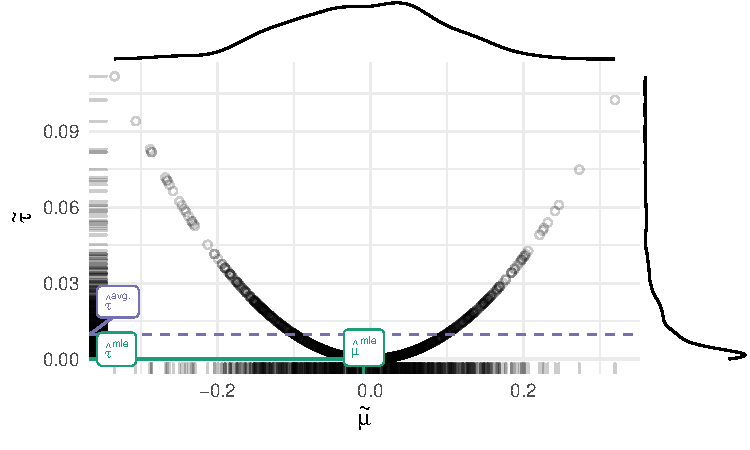
\includegraphics[width=.85\linewidth]{figs/intuition-1.pdf}
  \caption{Simulation 1 of 1,000}
  \label{fig:int1}
\end{subfigure}%
\begin{subfigure}{.5\textwidth}
  \centering
  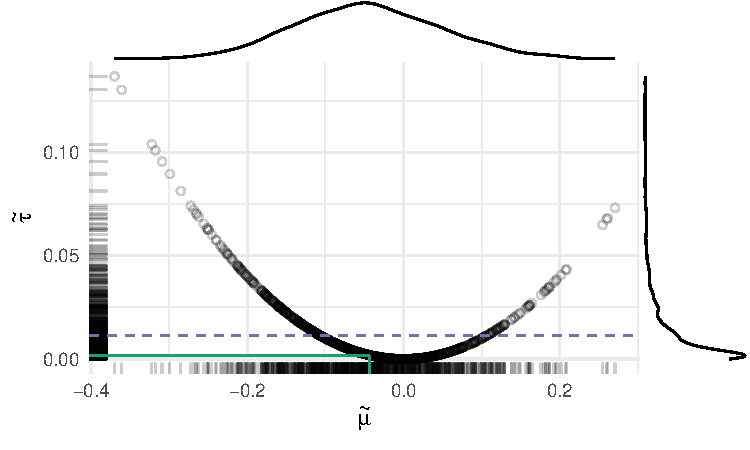
\includegraphics[width=.85\linewidth]{figs/intuition-2.pdf}
  \caption{Simulation 2 of 1,000}
  \label{fig:int2}
\end{subfigure}
\begin{subfigure}{.5\textwidth}
  \centering
  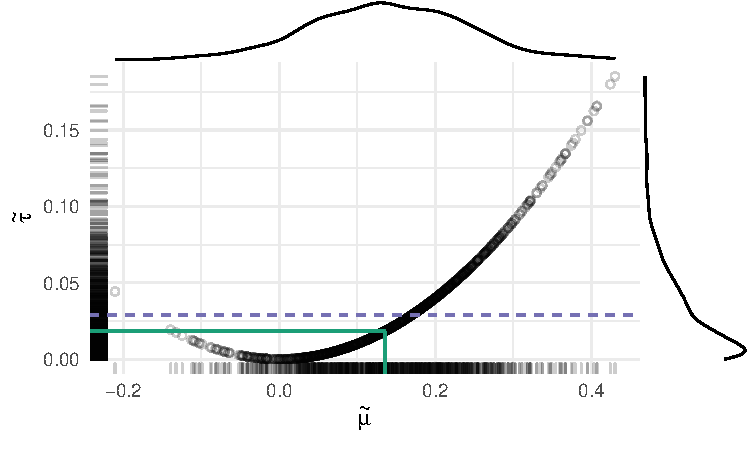
\includegraphics[width=.85\linewidth]{figs/intuition-3.pdf}
  \caption{Simulation 3 of 1,000}
  \label{fig:int3}
\end{subfigure}%
\begin{subfigure}{.5\textwidth}
  \centering
  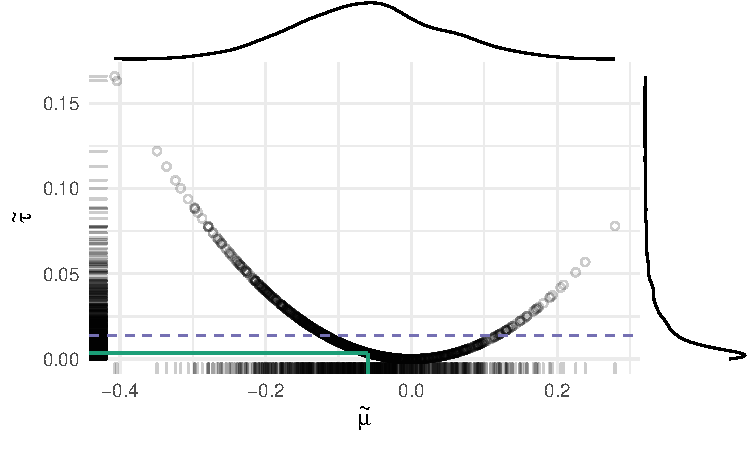
\includegraphics[width=.85\linewidth]{figs/intuition-4.pdf}
  \caption{Simulation 4 of 1,000}
  \label{fig:int4}
\end{subfigure}

\vspace{.1in}
\caption{Four figures illustrating the relationship between $\hat{\tau}^\text{mle}$ and $\hat{\tau}^\text{avg}$ described by Lemma \ref{lem:direction} and Theorem \ref{thm:direction}.}
\label{fig:int}
\end{figure}


Second, to find $\hat{\tau}^\text{mle}$, we simply transform $\hat{\mu}^\text{mle}$ directly using $\hat{\tau}^\text{mle} = \left( \hat{\mu}^\text{mle} \right) ^2$. The solid green lines show this transformation. Notice that $\hat{\tau}^\text{mle}$ corresponds approximately to the mode of the density plot of $\tilde{\tau}$ along the right side of the plot, which falls closer to the true value $\tau(0) = 0$ than $\hat{\tau}^\text{avg}$. The convex transformation $\tau(\cdot)$ has the effect of lengthening the right tail of the distribution of $\tilde{\tau}$, pulling the average well above the mode. This provides the basic intuition for Lemma \ref{lem:direction}.

Figures \ref{fig:int2}-\ref{fig:int4} repeat this process three more times to give some sense of how the dynamic changes for different samples. In each case, the story is similar---the convex transformation stretches the distribution of $\tilde{\tau}$ to the right, which pulls $\hat{\tau}^\text{avg}$ above $\hat{\tau}^\text{mle}$.

We repeat this process to produce 1000 estimates of $\hat{\mu}^\text{mle}$, $\hat{\tau}^\text{mle}$, and $\hat{\tau}^\text{avg}$.
Figure \ref{fig:int-samp} shows the density plots for the three empirical sampling distributions. As we would expect, $\hat{\mu}^\text{mle}$ is unbiased with a standard error of $\frac{1}{\sqrt{n}} = \frac{1}{\sqrt{100}} = \frac{1}{10}$. Both $\hat{\tau}^\text{mle}$ and $\hat{\tau}^\text{avg}$ are biased upward, but $\hat{\tau}^\text{avg}$ is more so. Theorem \ref{thm:direction} shows why this must be the case.

\begin{figure}[h]
\begin{center}
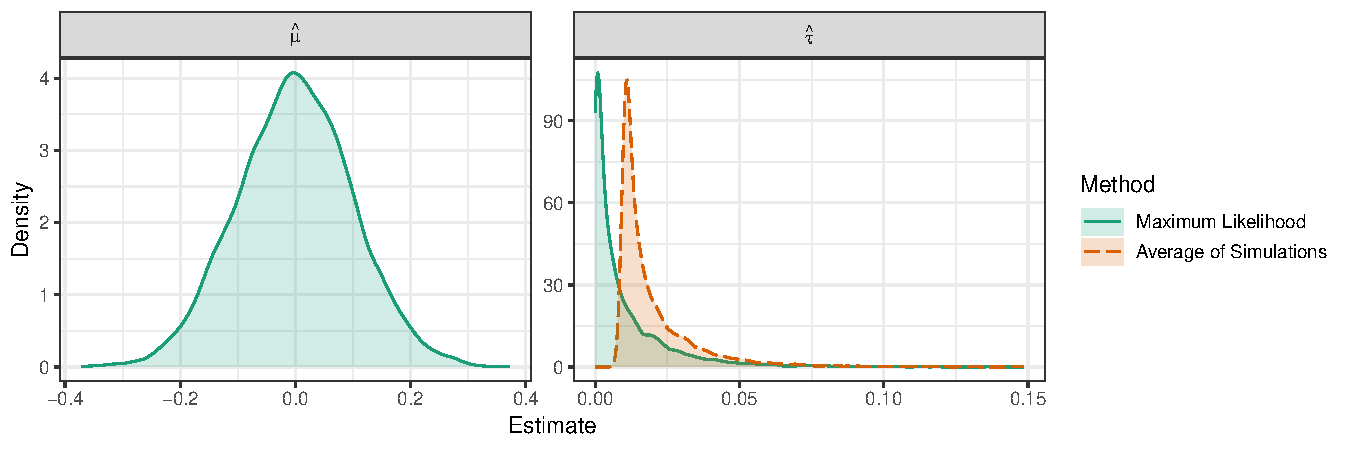
\includegraphics[scale = 0.75]{figs/intuition-sampling.pdf}\\
\vspace{.1in}
\caption{The sampling distributions of $\hat{\beta}^\text{mle}$, $\hat{\tau}^\text{mle}$, and $\hat{\tau}^\text{avg}$.}\label{fig:int-samp}
\end{center}
\end{figure}

\subsection*{Using the Law of Iterated Expectations}

We can also develop the intuition using a more mathematical approach via the law of iterated expectations. For this it helps if we alter the notation slightly, making two implicit dependencies explicit. We explain each change below and use the alternate, more expansive notation only in this section.

The law of iterated expectations states that $\E_Y \left( \E_{X \mid Y}(X \mid Y) \right) = E_X(X)$, where $X$ and $Y$ represent random variables. The three expectations occur with respect to three different distributions: $\E_Y$ denotes the expectation w.r.t. the marginal distribution of $Y$, $\E_{X \mid Y}$ denotes the expectation w.r.t. the conditional distribution of $X \mid Y$, and $\E_X$ denotes the expectation w.r.t. the marginal distribution of $X$.

Outside of this section, we realize that the distribution of $\tilde{\beta}$ depends on $\hat{\beta}^\text{mle}$ and could be written as $\tilde{\beta} \mid \hat{\beta}^\text{mle}$. To remain consistent with previous work, especially \cite{KingTomzWittenberg2000} and \cite{Herron1999}, we simply use $\tilde{\beta}$ to represent $\tilde{\beta} \mid \hat{\beta}^\text{mle}$. The definition of $\tilde{\beta}$ makes this clear. In this section only, we use $\tilde{\beta} \mid \hat{\beta}^\text{mle}$ to represent the conditional distribution of $\tilde{\beta}$ and $\tilde{\beta}$ to represent the \underline{un}conditional distribution of $\tilde{\beta}$. Intuitively, one might imagine (1) generating a data set $y$, (2) estimating $\hat{\beta}^\text{mle}$, and (3) simulating $\tilde{\beta} \mid \hat{\beta}^\text{mle}$. If we do steps (1) and (2) just once, but step (3) repeatedly, then we have a sample from the conditional distribution $\tilde{\beta} \mid \hat{\beta}^\text{mle}$. If we do steps (1), (2), and (3) repeatedly, then we have a sample from the \underline{un}conditional distribution $\tilde{\beta}$. The unconditional distribution will help us understand the nature of the excessive transformation-induced $\tau$-bias.\footnote{More technically, we could also define the relevant distributions hierarchically. First, we have $\hat{\beta}^\text{mle} \sim s(\beta)$, where $s(\beta)$ represents the sampling distribution of $\hat{\beta}$. Then we have $\tilde{\beta} \sim MVN \left[ \hat{\beta}^{\text{mle}}, \hat{V} \left( \hat{\beta}^{\text{mle}} \right) \right]$. {\color{red} HOLGER: I would drop this footnote; I don't think it adds much.}}

Applying the law of iterated expectations, we obtain $\E_{\tilde{\beta}} \left( \tilde{\beta} \right) = \E_{\hat{\beta}^\text{mle}}\left( \E_{\tilde{\beta} \mid \hat{\beta}^\text{mle}} (\tilde{\beta} \mid \hat{\beta}^\text{mle}) \right)$. The three identities below connect the three key quantities from Theorem \ref{thm:direction} to three versions of $\E_{\hat{\beta}^\text{mle}}\left( \E_{\tilde{\beta} \mid \hat{\beta}^\text{mle}} (\tilde{\beta} \mid \hat{\beta}^\text{mle}) \right)$, with the transformation $\tau(\cdot)$ applied at different points.

\begin{alignat}{2}
 \color{color1} \tikzmark{MarkA}\tau \left[ \normalcolor \E_{\hat{\beta}^\text{mle}}\left( \E_{\tilde{\beta} \mid \hat{\beta}^\text{mle}} \left( \tilde{\beta} \mid \hat{\beta}^\text{mle} \right) \right) \color{color1} \right] \normalcolor =&  \tau \left[ \E_{\tilde{\beta}} \left( \tilde{\beta} \right) \right] = \tau \left[\E \left( \hat{\beta}^\text{mle} \right) \right]\text{,} \label{eqn:true}\\
 \E_{\hat{\beta}^\text{mle}}\left( \color{color1} \tikzmark{MarkB}\tau\tikzmark{MarkC} \left[ \normalcolor \E_{\tilde{\beta} \mid \hat{\beta}^\text{mle}} \left( \tilde{\beta} \mid \hat{\beta}^\text{mle} \right) \color{color1} \right] \normalcolor \right)  =&  \E_{\hat{\beta}^\text{mle}} \left( \tau \left[\hat{\beta}^\text{mle} \right] \right) =  \E_{\hat{\beta}^\text{mle}} \left(\hat{\tau}^\text{mle} \right) \text{, and} \justif{\quad}{$\longleftarrow~$ Switch $\tau$ and an $\E$ once.} \label{eqn:mle}\\
\E_{\hat{\beta}^\text{mle}}\left( \E_{\tilde{\beta} \mid \hat{\beta}^\text{mle}} \left( \color{color1} \tikzmark{MarkD}\tau \left[ \normalcolor \tilde{\beta} \mid \hat{\beta}^\text{mle} \color{color1} \right] \normalcolor \right) \right)  =&
\E_{\tilde{\beta}} \left( \tau \left[\tilde{\beta} \right] \right)  =
\E_{\tilde{\beta}} \left(\hat{\tau}^\text{avg} \right) \text{.}\justif{\quad}{$\longleftarrow~$ Switch $\tau$ and an $\E$ again.}\label{eqn:avg}\DrawBox{red}{blue}
\end{alignat}

If we subtract Equation \ref{eqn:mle} from Equation \ref{eqn:true} we obtain the transformation-induced $\tau$-bias in $\hat{\tau}^\text{mle}$ (see Equation \ref{eqn:ti-bias} for the definition of transformation-induced $\tau$-bias).
To move from Equation \ref{eqn:true} to Equation \ref{eqn:mle} we must swap $\tau(\cdot)$ with an expectation once. This implies that, if $\tau(\cdot)$ is convex, Equation \ref{eqn:mle} must be greater than Equation \ref{eqn:true}.
This, in turn, implies that the bias is positive.

To obtain the transformation-induced $\tau$-bias in $\hat{\tau}^\text{avg}$ we must subtract Equation \ref{eqn:avg} from Equation \ref{eqn:true}. But to move from Equation \ref{eqn:true} to Equation \ref{eqn:avg} we must swap $\tau(\cdot)$ with an expectation \emph{twice}. Again, if $\tau(\cdot)$ is convex, then Equation \ref{eqn:avg} must be greater than Equation \ref{eqn:true}. However, because we expect $\hat{\beta}^\text{mle}$ and $\tilde{\beta} \mid \hat{\beta}^\text{mle}$ to have similar distributions, we should expect the additional swap to roughly double the bias in $\hat{\tau}^\text{avg}$ compared to $\hat{\tau}^\text{avg}$.

\section*{Illustrative Simulations}

\subsection*{Marginal Effects in Poisson Regression}

As an illustration, consider the Poisson regression model $y_i \sim \text{Poisson}(\lambda_i)$, where $\lambda_i = e^{(-2 + x_i)}$ for $i \in \{1, 2,\ldots, 100\}$. To create $x_i$ we take $100$ i.i.d.\@ draws from a standard normal distribution. Assume that the researcher wants to estimate the instantaneous marginal effect of $x$ on $\E(y)$, so that $\tau(\beta) = \frac{d \E (y)}{dx} = e^{(\beta_{cons} + \beta_x x)}$ for $x$ ranging from $-3$ to $+3$.

Following the procedures discussed above, we generate 10,000 data sets and use each data set to estimate $\hat{\tau}^\text{mle}$ and $\hat{\tau}^\text{avg}$.
Note that the transformation is convex, so according to Theorem \ref{thm:direction} the transformation-induced $\tau$-bias in both $\hat{\tau}^\text{mle}$ and $\hat{\tau}^\text{avg}$ will be positive.
The rule of thumb suggests about twice as much bias in $\hat{\tau}^\text{avg}$ as in $\hat{\tau}^\text{mle}$.

Figure \ref{fig:poisson-mcs} shows the transformation-induced $\tau$-bias in $\hat{\tau}^\text{avg}$ and $\hat{\tau}^\text{mle}$ compared to the true value $\tau(\beta)$. Notice three features of this plot. First, the bias is substantial. The relative size of the bias varies, but when the true marginal effect is greater than 0.5, the average transformation-induced $\tau$-bias in $\hat{\tau}^\text{mle}$ is about $\frac{1}{3}$ the size of the true effect. [{\color{red} HOLGER: I think these numbers are still off.}] For $\hat{\tau}^\text{avg}$, the bias is about $\frac{3}{4}$ the size of the true effect. Second, notice that the bias occurs in the expected direction. Because the transformation $\tau(\beta) = \frac{d \E (y)}{dx} = e^{(\beta_{cons} + \beta_x x)}$ is convex, the bias is positive. Third, notice that the bias in $\hat{\tau}^\text{avg}$ is about twice as large as the bias in $\hat{\tau}^\text{mle}$, as the rule of thumb suggests.

\begin{figure}[h!]
\begin{center}
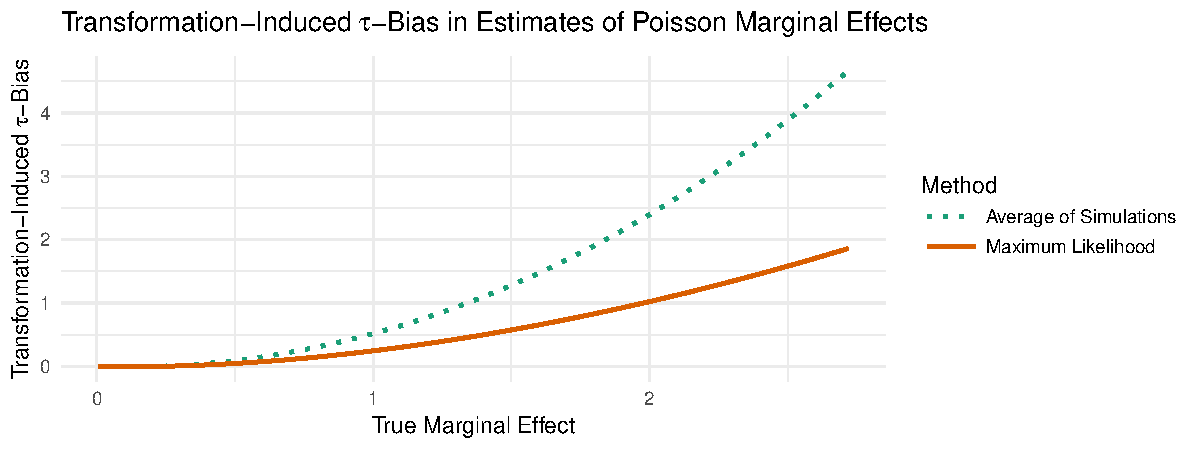
\includegraphics[scale = 0.65]{figs/poisson-mcs.pdf}
\vspace{.1in}
\caption{This figure shows the bias in the estimates of the marginal effects in a Poisson regression model. Notice that the convex transformation $\tau(\beta) = \frac{d \E (y)}{dx} = e^{(\beta_{cons} + \beta_x x)}$ creates a positive bias (see Theorem \ref{thm:direction}) and that the bias in $\hat{\tau}^\text{avg}$ is about twice as large as the bias in $\hat{\tau}^\text{mle}$ (compare Equations \ref{eqn:avg-approx} and \ref{eqn:mle-approx}).}\label{fig:poisson-mcs}
\end{center}
\end{figure}

\section*{Example: Supreme Court Decisions}

To unify explanation of U.S. Supreme Court decisions, \cite{GeorgeEpstein1992} fit a single probit model that combines the legal and extralegal models of Court decision-making to a data set of 64 decisions.
The authors model the probability of a conservative decision as a function of whether the Solicitor General filed an Amicus brief (SG = 1) or not (SG = 0) and 10 other explanatory variables.
See \cite{GeorgeEpstein1992} for the more details of the model.

We use this model illustrate the potential impact of using the simulation average rather than the maximum likelihood estimate of the quantity of interest.
We focus on two potential quantities of interest: the probability of a conservative decision and the effect of the Solicitor General filing a brief.
Table \ref{tab:ge-qi} summarizes these quantities of interest.

\begin{table}[h!]
\centering
\caption{This table provides the details of the quantities of interest from George and Epstein's (1992) model of U.S. Supreme Court decisions.}
\label{tab:ge-qi}
\footnotesize
\begin{tabular}{@{} m{5cm} m{4cm} m{2.5cm}m{4cm}@{}}
\toprule
Description                                                                       & Notation                                                  & Change in Key Explanatory Variable               & Values for Other Explanatory Variables \\ \midrule
probability of a conservative decision                                            & $\tau(\beta) = \Phi(X_c \beta)$                           & none                                             & every observed combination   \\\hline
effect of a Solicitor General brief on the probability of a conservative decision & $\tau(\beta) = \Phi(X_\text{high} \beta) - \Phi(X_\text{low}\beta)$ & for $X_\text{high}$, SG = 1, and for $X_\text{low}$, SG = 0 & every observed combination   \\ \bottomrule
\end{tabular}
\end{table}

For each quantity of interest, we compute an estimate using the average of simulation and maximum likelihood.
First, we use both the average of simulations and maximum likelihood to estimate the probability of a conservative decision for each combination of explanatory variables included in the data set.
Second, we use both approaches to estimate the effect of a Solicitor General brief on the probability of a conservative decision.
We define this effect as the \textit{difference} in the probability of a conservative decision for each observation in the data set, if that observation changed from one in which the Solicitor General \emph{did not} file a brief (SG = 0) to one in which the Solicitor General \emph{did} file a brief (SG = 1).

Figure \ref{fig:ge} compares the estimates.
First, consider the estimates of the probability of a conservative decision in Figure \ref{fig:ge1}.
The pattern is clear: when the chance of a conservative decision is less than 50\%, the average of the simulations is too large.
In this region, the transformation (the normal cdf) is convex.
When the chance of a conservative decision is greater than 50\%, the average of the simulations is too small.
In this region, the transformation is concave.
When the chance of a conservative decision is closer to 50\%, the differences between the average of the simulations and the maximum likelihood estimate are smaller, because the transformation is more linear in this area.
The same is true for chances close to 0\% and 100\%.

Further, some of the differences are quite large.
For example, when maximum likelihood suggests a chance of about 5\%, the average of the simulation suggests a chance of about 10\%.
This difference may seem small at first (i.e., only 5 percentage points), but the average of simulations is about \textit{double} the maximum likelihood estimate.


\begin{figure}[h!]
\begin{subfigure}{.5\textwidth}
  \centering
  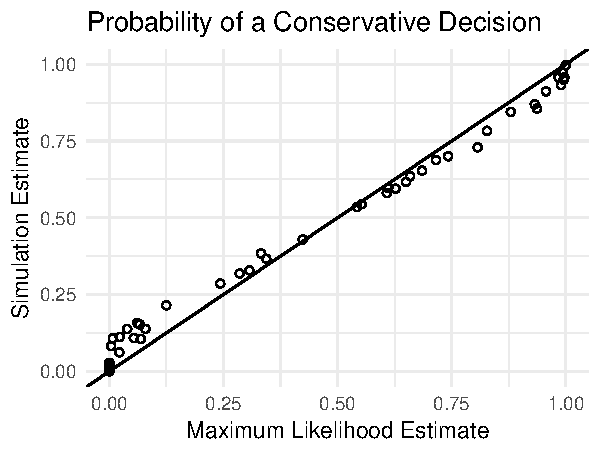
\includegraphics[width=.8\linewidth]{figs/ge-pr.pdf}
  \caption{}
  \label{fig:ge1}
\end{subfigure}%
\begin{subfigure}{.5\textwidth}
  \centering
  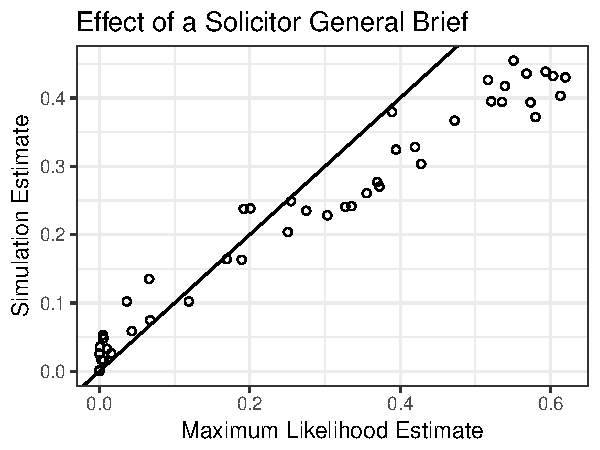
\includegraphics[width=.8\linewidth]{figs/ge-fd.pdf}
  \caption{}
  \label{fig:ge2}
\end{subfigure}
\caption{The figure shows the relationship between the simulation average and the maximum likelihood estimate two the quantities of interest. The left panel (a) shows the probability of a conservative decision. Notice that the simulation average tends falls about the maximum likelihood estimate when the probability is low--where the transformation is convex--and below the maximum likelihood estimate when the probability is high--where the transformation is concave. The right panel (b) shows the effect of a brief by the Solicitor General on the probability of a conservative decision.}
\label{fig:ge}
\end{figure}

Now consider the estimates of the effect of the Solicitor General filing an Amicus brief in Figure \ref{fig:ge2}.
The largest differences appear in the upper-right corner of the plot.
For this group of observations, the average of simulations suggests than a brief from the Solicitor General increases the chance of a conservative decision by about 40 percentage points.
On the other hand, the maximum likelihood estimate suggests an increase of about 60 percentage points.
This difference is certainly meaningful---the maximum likelihood estimate is 50\% larger than the average of the simulations.

\subsection*{A Note on \cite{HanmerKalkan2013}}

\cite{HanmerKalkan2013} discusses two approaches to computing quantities of interest: the more commonly used {\it average-case} approach and their recommended {\it observed-value} approach. With either approach, researchers estimate the quantity of interest as a key explanatory variable changes its value. However, in non-linear models researchers must also deal with the other explanatory variables in the model, because these variables alter the quantity of interest. The average-case approach sets the other explanatory variables to central values such as the mean, median, or mode. \cite{HanmerKalkan2013} in contrast suggests estimating the quantity of interest for all sample observations, leaving their explanatory variables except for the key variable of interest at their observed values, and then averaging the estimates across the sample. Here, this choice is implicitly part of the transformation $\tau(\cdot)$, so their (compelling) argument does not undermine or enhance our own.\footnote{We generally agree with the arguments in favor of the observed-value approach but recommend that researchers plot the distribution of quantities of interest in addition to providing a summary measure such as their average. See Ai and Norton (2003) for examples.}

Because researchers have not drawn a sharp conceptual distinction between using the average of simulation draws and using the ML invariance property, \cite{HanmerKalkan2013} does not discuss this choice. Since it explicitly builds on \cite{KingTomzWittenberg2000}, we interpreted \cite{HanmerKalkan2013} as relying on the average of simulation draws when computing quantities of interest. The replication archive for the article confirms that this is indeed the case.

The important point is this: \cite{HanmerKalkan2013} draws a distinction between the average-case and observed-value approaches to computing
quantities of interest. Our paper draws a distinction between estimating quantities of interest (whether average-case or observed-value based) using the average of simulated draws and using the ML invariance property. Regardless of whether researchers use the average-case approach or the observed-value approach, the average of simulation draws will lead to estimates that generally will suffer from bias that can easily be avoided by relying on the ML invariance property instead.\footnote{\color{red} HOLGER: Do we want to say anything about what to do when using non ML estimators?}

\section*{Conclusion}

Many political scientists turn to \cite{KingTomzWittenberg2000}'s seminal paper when seeking advice on how to interpret, summarize, and present empirical results. By highlighting the importance of reporting substantively meaningful quantities of interest accompanied by valid measures of statistical uncertainty, \cite{KingTomzWittenberg2000} has significantly improved empirical research in political science and neighboring disciplines. However, depending on the statistical software used, political scientists following \cite{KingTomzWittenberg2000}'s advice will estimate quantities of interest either with the average of simulation draws (e.g., CLARIFY in Stata, Zelig in \texttt{R}) or relying on the ML invariance property (e.g., margins in Stata and \texttt{R}). In practice, researchers' choice between the two approaches seems idiosyncratic rather than principled. As far as we can tell, it is largely a function of which software package a researcher prefers to use, with little thought given to differences in the underlying statistical machinery. Even the methodological literature has failed to pay attention to potential differences between the two approaches to estimating quantities of interest.

\cite{Rainey2017} stresses the importance of transformation-induced bias, which originates in the non-linear transformation of model coefficient estimates into estimated quantities of interest. As shown by \cite{Rainey2017}, such transformation-induced biases will be large when standard errors are large or when the transformation of the model coefficients into quantities of interest is highly non-linear. Our paper shows that when we use the average of simulation draws we incur about \textit{twice} as much bias as when we rely on the ML invariance property. The good news is that the fix is easy: do not use the average of simulation draws to estimate quantities of interest. Instead, simply plug model coefficients into the transformation to obtain an estimate of the quantity of interest. We recommend that statistical software does this by default.\footnote{Based on communications with Christopher Gandrud, a member of the Zelig Core Team, it appears that Zelig sometimes uses the median of the simulation draws as point estimator (as opposed to the mean). We were not able to find any information in the Zelig documentation (Choirat et al.\@ 2017) for when that might happen. Note that the median of the simulation draws does not correspond to the estimator based on the ML invariance property unless the transformation is monotonic. (Even then stochastic simulation would introduce Monte Carlo error that could easily be avoided by relying on the ML invariance property in the first place.) To see this revisit the previous example where $\tau(\mu) = \mu^2.$ Imagine the best-case scenario in which $\hat{\mu}^\text{mle} = 0$, so that the estimator based on the ML invariance property is unbiased. Even then simulated draws of the quantity of interest will almost surely be greater than zero. Taking either the mean or the median of the simulated draws will result in a biased estimator of the quantity of interest.}


Finally, if researchers use the ML invariance property to estimate quantities of interest, how should they conduct statistical inference? Commonly employed approaches include the delta method, stochastic simulation (but using the ML invariance property for the point estimator, as suggested by Herron (1999)), or the bootstrap (e.g., Efron and Tibshirani 1993). Krinsky and Robb (1991) presents some limited Monte Carlo evidence that these approaches lead to similar inferences but a more detailed examination of this question is, to the best of our knowledge, still missing from the literature.

\singlespace
%\newpage
\small
\bibliographystyle{apsr_fs}
\bibliography{/Users/carlislerainey/Dropbox/papers/bibliography/bibliography.bib}

\end{document}
